\documentclass[conference]{IEEEtran}
\IEEEoverridecommandlockouts
\usepackage{cite}
\usepackage{amsmath,amssymb}
\usepackage{graphicx}
\usepackage{booktabs}
\usepackage{xcolor}
\usepackage{url}
\usepackage[hidelinks]{hyperref}
\graphicspath{{figures/}}
\newcommand{\D}{\ensuremath{D}}

\begin{document}

\title{When We Edit an AI's Thoughts, Is It ``Doing'' or ``Seeing''?\\
\large Activation Patching Makes Language Models Infer the Cause of the Patched Fact}

\author{\IEEEauthorblockN{Pranav Kalla (PES1UG24AM197) \quad Pranav Prabhakar (PES1UG24AM463)}
\IEEEauthorblockA{Team Ground Truth --- Advanced Data Analytics, Jackfruit Project\\
Department of Computer Science and Engineering (AI \& ML), PES University, Bengaluru, India}}

\maketitle

\begin{abstract}
Activation patching is an intervention on a network. Is it also an intervention in the world the network represents? Using Pearl's distinction between \emph{seeing} and \emph{doing}, we compare patched facts against each model's own behaviour when it reads a fact (``the road was icy'') and when it reads the same fact as imposed (``a pipe burst and the water froze, so the road was icy''). We built a dataset of 79 causal scenarios (1{,}896 stories) in three structures (chains, colliders, forks) and tested three model families (Qwen3-4B, Llama-3.2-3B, Gemma-2-2B) and two answer formats. A patched fact is treated as evidence: the model infers the fact's usual cause and explains away competing causes, with a do-likeness score near 0 wherever patches work. The cause is not copied in with the patch. We then ask whether a patch can carry an intervention. Copying the fact from the imposed story changes nothing through most of the network and moves the model only partly towards doing in the last layers where patches work; conversely, the imposed story stays do-like when its fact word is overwritten. Both results were confirmed in a test with predictions written in advance. Knowledge of \emph{how} a fact came about is held at the cause words, not with the fact. We also show that yes/no probes of steered models can mistake a general bias towards ``Yes'' for a causal effect.
\end{abstract}

\begin{IEEEkeywords}
interpretability, activation patching, causal inference, do-calculus, large language models, explaining away
\end{IEEEkeywords}

%=====================================================================
\section{Introduction}
Interpretability research edits the hidden states of language models and reads the consequences causally. Activation patching copies a state from one run into another \cite{vig2020,meng2022,heimersheim2024}; causal abstraction treats such an interchange as an intervention on a high-level variable \cite{geiger2025}; a recent position paper places patching on the interventional rung of Pearl's ladder \cite{joshi2026}. At the level of the network this is right by construction: we set a state, whatever the earlier layers computed.

But the network also represents a world, and in that world the same edit can mean two things. Pearl \cite{pearl2009} separates \textbf{seeing} from \textbf{doing}. If you \emph{see} that the road is icy, you infer that it probably snowed. If someone floods the road and lets it freeze, the road is just as icy, but you learn nothing about snow. When we patch ``the road is icy'' into a model, which of the two has happened in the story it is tracking?

One answer is easy to guess: the layers after the patch were trained only on states that came from reading text, and cannot tell where a state came from, so they should treat a patched fact as evidence. If so, it matters: the effects of a patch mix the consequences of a fact with inferences about its causes, and ``patching $X$ changed $Y$'' does not mean ``$X$ causes $Y$ in the model's world''. Yet the guess has not been tested, and our first attempt shows how easily a test goes wrong: steering vectors appeared to act as evidence, but only because they pushed every answer towards ``Yes'' (Sec.~\ref{sec:steer}).

We test the guess with each model's own behaviour as the yardstick and score an edit by where it falls between seeing and doing (do-likeness \D; 0 = seeing, 1 = doing). Our contributions:
\begin{enumerate}
\item A behavioural test of whether a hidden-state edit acts as seeing or doing in the model's represented world, with a score normalised by effect size and a fixed rule for when an edit is strong and specific enough to score.
\item Evidence that patched facts are treated as evidence across 79 scenarios, three causal structures, three model families and two answer formats, with confirmatory runs on held-out scenarios and written predictions.
\item A confirmed finding about where intervention knowledge lives: at the cause words, reaching the fact's position only in the last working layers and only partly.
\item A methodological warning: yes/no probes of edited models need unrelated-question controls.
\end{enumerate}

%=====================================================================
\section{Related Work}
\textbf{Patching as intervention.} Causal mediation analysis and activation patching locate where information matters in a network \cite{vig2020,meng2022,heimersheim2024}, and causal abstraction formalises interchange interventions as interventions on high-level variables \cite{geiger2025}. Joshi et al.\ \cite{joshi2026} argue that interpretability claims should state their causal estimand and class patching as interventional. Work on the pitfalls of patching has focused on the network level: subspace patches can act through dormant directions \cite{makelov2024}, and learned subspace interventions can overstate effects \cite{tanyel2026}. We do not dispute the network-level reading; we ask what the edit amounts to in the world the model represents.

\textbf{Edits as belief change.} Bigelow et al.\ \cite{bigelow2025} model steering as a shift in the model's prior over latent concepts and in-context examples as accumulating evidence. We test directly whether downstream reasoning after a \emph{patch} follows the observational or the interventional pattern, against the model's own text behaviour.

\textbf{Seeing and doing in LLM behaviour.} Behavioural studies test whether LLMs reason correctly about observations and interventions in text, including collider reasoning and explaining away \cite{dettki2025,dettki2026,feng2026}. They do not edit internal states. We use the same distinction as a measuring stick for edits.

\textbf{Knowledge editing and binding.} RippleEdits \cite{cohen2024} asks whether weight edits propagate \emph{forward} to implied facts; we look \emph{backward}, at whether an edited fact changes beliefs about its causes. Prakash et al.\ \cite{prakash2026} trace how models bind and look up beliefs across token positions; our second finding is of this kind.

%=====================================================================
\section{Dataset}
We wrote a template generator (released with the code) that produces short causal stories in three structures (Table~\ref{tab:data}). Each scenario is told in 24 surface variants (6 opening lines $\times$ 4 character names), giving 1{,}896 stories. Variants 16--23 are held out for every score; variants 0--15 were used only to learn steering directions and, later, as fresh items for the pre-registered test (Sec.~\ref{sec:ds2}).

\begin{table}[t]
\caption{Dataset. Example: cause $\rightarrow$ fact $\rightarrow$ effect.}
\label{tab:data}
\centering\small
\begin{tabular}{@{}lcl@{}}
\toprule
Structure & Scen. & Example \\
\midrule
Chain $A\!\rightarrow\!B\!\rightarrow\!C$ & 45$^\ast$ & snow $\to$ road icy $\to$ bus late \\
Collider $A\!\rightarrow\!C\!\leftarrow\!B$ & 19 & ``$C$ happens if $A$ or $B$'' \\
Fork $B\!\leftarrow\!A\!\rightarrow\!C$ & 15 & cold $\to$ pond frozen; cold $\to$ coats \\
\bottomrule
\multicolumn{3}{@{}l@{}}{\footnotesize $^\ast$20 exploration + 25 confirmation, written after the analysis was fixed.}
\end{tabular}
\end{table}

The edited fact is one sentence that comes in \textbf{minimal pairs} differing in one word: \emph{true} (``The road was \textbf{icy}.''), \emph{false} (``\dots\textbf{dry}.'') and \emph{neutral} (``\dots\textbf{long}.'', an irrelevant property). The neutral version is the \textbf{base} story every patch is applied to. A fourth, \textbf{do} version states the same fact as imposed by an outside agent: ``A broken water pipe had flooded the road overnight and the water froze, so the road was icy.'' Colliders add versions stating the other cause $A$, to measure explaining away. The cause is never mentioned in any story; it is only asked about. Each story is probed with five yes/no questions: the cause, the effect (or sibling effect in forks), the fact itself and three unrelated \emph{filler} questions (``Was there a cat nearby?'', ``Did someone in the story have a brother?'', ``Was a radio playing?'').

%=====================================================================
\section{Method}
\subsection{Models and belief readout}
We study three base models: Qwen3-4B-Base (36 layers; main model, chosen in a pilot over Pythia-1.4B, Gemma-2-2B and Qwen2.5-1.5B/3B for the clearest seeing/doing separation in text), Llama-3.2-3B (28 layers) and Gemma-2-2B (26 layers). Qwen and Llama run in float16 with a float32 unembedding; Gemma in bfloat16 with eager attention and its logit soft-cap. Each probe is a 2-shot prompt followed by the test story and a question; the model's \textbf{belief} is
\begin{equation}
b = \log P(\text{`` Yes''}) - \log P(\text{`` No''}).
\end{equation}
All shifts are \textbf{filler-corrected}: from the change in a question's belief we subtract the mean change on the three fillers, removing a general drift towards ``Yes''.

\subsection{Seeing vs doing from text, and the score \D}
Reading the true fact (\emph{see}) should raise belief in both the cause and the effect; reading it as imposed (\emph{do}) should raise the effect but leave the cause alone. For every scenario we measure the shifts $\Delta$cause and $\Delta$effect from the base story and take $r = \Delta\text{cause}/\Delta\text{effect}$, which normalises away how strongly the fact itself was pushed. A scenario is \textbf{valid} for a model only if the model separates the two cases in text: $\Delta$cause(see) $>0.5$, $\Delta$effect(see) $>0.5$, $\Delta$effect(do) $>0.5$ and $r_\text{see}-r_\text{do}>0.25$ (fixed before any edit was scored). For an edit,
\begin{equation}
D = \frac{r_\text{see} - r_\text{edit}}{r_\text{see} - r_\text{do}},
\end{equation}
so $D=0$ means the edit behaves like reading the fact and $D=1$ like an outside intervention. $D$ is scored only where the edit moves the effect by at least half as much as reading does. In colliders $r=\Delta B/\Delta C$; in forks $r=\Delta\text{cause}/\Delta\text{mediator}$, and the sibling effect gets a second score $D_\text{sib}$.

\subsection{Interventions on the hidden state}
\textbf{Steering (first attempt).} The mean difference of residual states between true and false stories (training variants) was added, scaled by $\alpha\in[1,16]$, at one layer and at the fact token, the tokens after it, or the answer token.

\textbf{Activation patching (main method).} We run a \emph{source} story, record the residual stream (output of block $L$) and write it into the base story at the same layer. A \emph{word} patch replaces the last token of the key word (``long''$\leftarrow$``icy''); a \emph{sentence} patch replaces that token through the end of the sentence. Sources (same surface variant as the target): \textbf{true} (the see story, the edit under test), \textbf{false} (must lower the fact's belief), \textbf{unrelated} (next valid scenario; controls for generic effects of patching) and \textbf{do} (the intervention story at the same word; Sec.~\ref{sec:ds}). Batches are left-padded with explicit position ids so a patch lands on the same token in every row.

\subsection{Pass rule, statistics and pre-registration}
A setting (layer $\times$ patch size) \textbf{passes} only if, over valid scenarios: the true patch moves the fact's filler-corrected belief by $\ge1.0$; it beats the unrelated patch by $>0.5$ in $\ge70\%$ of scenarios; the fillers move by $<0.5$; and the false patch moves the fact's belief below 0. \D\ is interpreted only at passing settings scored in at least 5 scenarios. We report medians over scenarios with 95\% bootstrap CIs (resampling scenarios); comparisons of two sources use paired differences and a sign-flip test. Before every confirmatory run we saved written predictions to a timestamped file (six files in all). Results that were not predicted are labelled exploratory.

%=====================================================================
\section{Results}
\begin{figure*}[t]
\centering
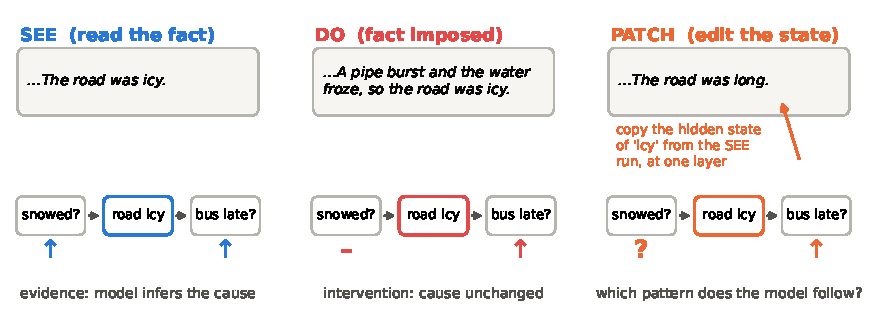
\includegraphics[width=0.78\textwidth]{fig_schematic.pdf}
\caption{Reading a fact (see) should raise belief in its cause and effect; an imposed fact (do) only in its effect. We ask which pattern the model follows when the fact's hidden state is copied into a story that does not state it.}
\label{fig:schematic}
\end{figure*}

\subsection{Steering looks seeing-like, but it is a yes-bias}\label{sec:steer}
Raw steering results suggested seeing: adding the ``icy'' direction raised belief in the cause. The filler questions exposed the problem (Fig.~\ref{fig:steer}). At layer 16 ($\alpha=4$, positions after the fact) the cause rose by 2.62 log-odds but the unrelated fillers rose by 3.04, and a direction from an unrelated scenario moved the answers about as much. After filler correction the best setting moved belief in the fact itself by only 0.89 (reading moves it by 4--5) and no setting passed the rule. We therefore switched to patching. \textbf{Lesson:} yes/no probes of an edited model need an unrelated-question control.

\begin{figure}[t]
\centering
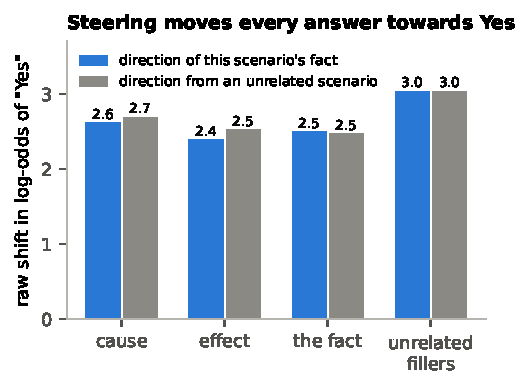
\includegraphics[width=0.85\columnwidth]{fig_steering.pdf}
\caption{Qwen3-4B steering at layer 16 ($\alpha=4$), raw shifts. The scenario's own direction and an unrelated one move cause, effect, fact and filler questions alike.}
\label{fig:steer}
\end{figure}

\subsection{Patches act as evidence}
In Qwen3-4B, patching the state of ``icy'' into ``The road was long'' makes the model infer snow exactly as reading ``icy'' does (Table~\ref{tab:main}, Fig.~\ref{fig:main}). All four predictions written before the confirmation run held. A denser sweep over the 30 valid scenarios shows the patch passing at every layer up to 17 and failing from 18, with median \D\ between $-0.13$ and $+0.15$ and intervals including 0 at every layer but one (layer 14 sentence, $-0.06$).

\begin{table}[t]
\caption{Patching chains in Qwen3-4B.}
\label{tab:main}
\centering\small
\begin{tabular}{@{}lcc@{}}
\toprule
 & Exploration (20) & Confirmation (25) \\
\midrule
Valid scenarios & 15 & 15 \\
Layers where patch passes & 0--15 & 0--15 \\
Fact shift (true patch) & $+4.4$ to $+4.8$ & $+4.0$ to $+4.5$ \\
True beats unrelated & 100\% & 100\% \\
Filler / false patch & $\approx0$ / $\approx-2$ & $\approx0$ / $\approx-2$ \\
Median \D, layers 0--12 & $-0.04$ to $+0.01$ & $-0.09$ to $+0.01$ \\
Patch fails from & layer 18 & layer 18 \\
\bottomrule
\end{tabular}
\end{table}

\begin{figure*}[t]
\centering
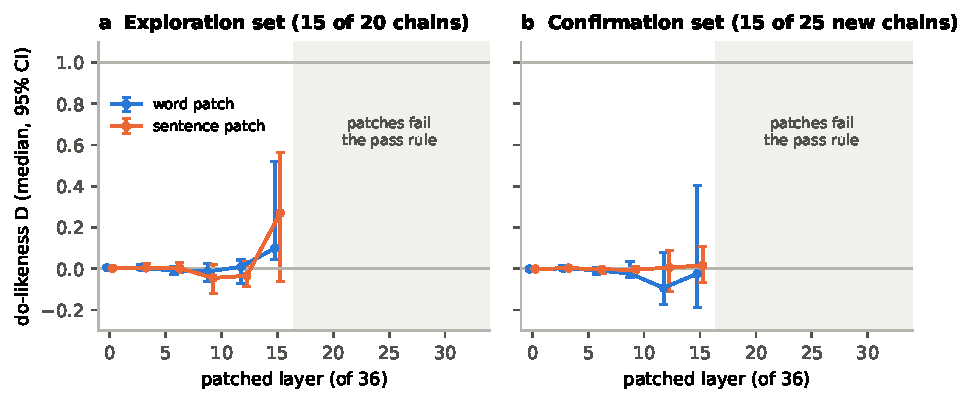
\includegraphics[width=0.8\textwidth]{fig_main.pdf}
\caption{Qwen3-4B: median \D\ (95\% CI) at layers where the patch passes, for word and sentence patches, in the exploration set and in the confirmation set written after the analysis was fixed.}
\label{fig:main}
\end{figure*}

\subsection{Colliders and forks}
\textbf{Colliders} ($A\to C\leftarrow B$). Observing $C$ should raise belief in $B$; then learning that $A$ happened should lower it again (explaining away). In text the interaction was positive in all 19 scenarios (17 passed our criteria). On the minimal-pair stories 12 scenarios pass the filters, with a text interaction of 1.10. Patching $C$'s state gives \D\ between $-0.02$ and $+0.05$ at layers 0--15, and an explaining-away interaction of 0.92--1.21 (CIs 0.49--1.70), the same size as when $C$ is read (Fig.~\ref{fig:coll}). An intervention on $C$ would give none, since it says nothing about $B$. All four predictions held.

\begin{figure*}[t]
\centering
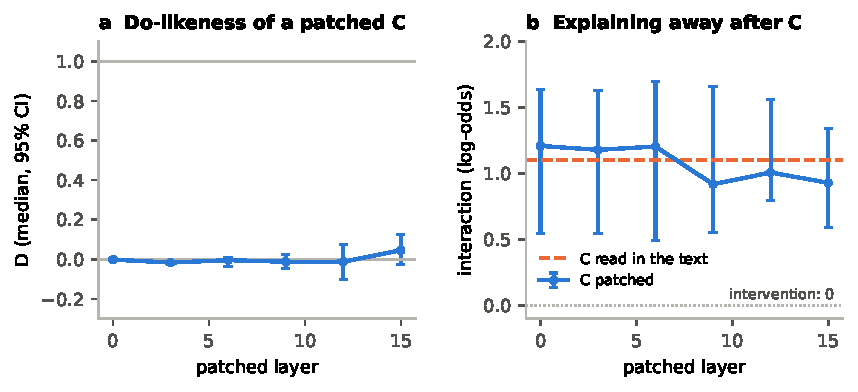
\includegraphics[width=0.78\textwidth]{fig_colliders.pdf}
\caption{Qwen3-4B colliders (12 scenarios). (a) Median \D\ of a patched $C$. (b) Explaining-away interaction after a patched $C$ vs after reading $C$; an intervention on $C$ would give 0.}
\label{fig:coll}
\end{figure*}

\textbf{Forks} (cold $\to$ frozen pond; cold $\to$ thick coats). Valid in 9/15 scenarios for both Qwen and Llama. Median \D\ for the cause is $-0.02$ to $+0.05$ at Qwen layers 0--12 and $0.00$ to $+0.11$ in Llama; the sibling effect is also inferred ($D_\text{sib}\le0.02$ in Qwen, $\le0.09$ in Llama). All fork predictions held.

\subsection{Replication across models and answer formats}
The result replicates in two further families (Table~\ref{tab:models}, Fig.~\ref{fig:models}). The patch controls hold in every model: true beats unrelated in 100\% of scenarios, false patches push belief down, fillers move by at most 0.21. Gemma-2-2B rarely separates seeing from doing in text, so it is tested on 12 scenarios only. In every model patches lose their effect at roughly 35--50\% of depth.

\begin{table}[t]
\caption{Chains across models.}
\label{tab:models}
\centering\small
\setlength{\tabcolsep}{3pt}
\begin{tabular}{@{}lcccc@{}}
\toprule
Model & Valid & Passes & Median \D & Stops \\
\midrule
Qwen3-4B & 30/45 & L0--17 & $-0.13$ to $+0.15$ & L18/36 \\
Llama-3.2-3B & 23/45 & L0--9 & $-0.03$ to $+0.01$\,(L0--6) & L12/28 \\
Gemma-2-2B & 12/45 & L0--6 & $-0.01$ to $+0.08$ & L9--12/26 \\
\bottomrule
\end{tabular}
\end{table}

\begin{figure*}[t]
\centering
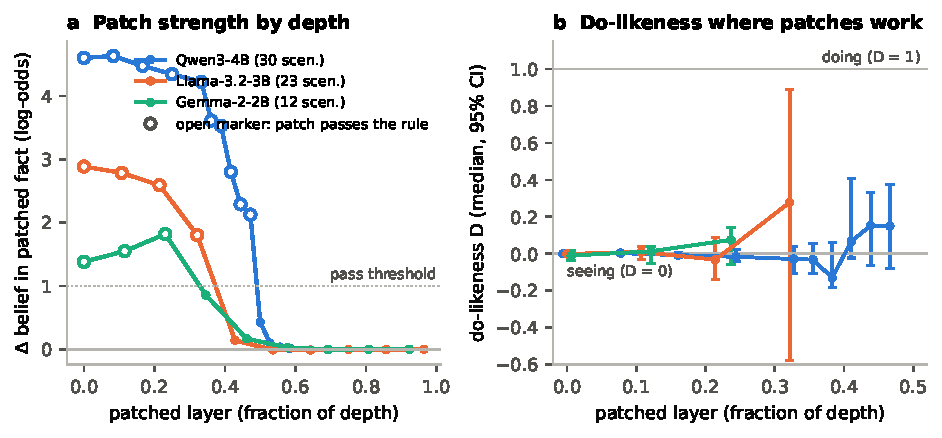
\includegraphics[width=0.8\textwidth]{fig_models.pdf}
\caption{(a) Shift in belief in the patched fact (true word patch, filler-corrected) by relative depth; open markers pass the fixed rule. (b) Median \D\ with 95\% CIs at passing layers scored in $\ge5$ scenarios.}
\label{fig:models}
\end{figure*}

\textbf{Answer format.} Rerunning Qwen with True/False answers ($b=\log P(\text{`` True''})-\log P(\text{`` False''})$, all references recomputed): 25/30 scenarios still pass the text filters; the patch passes at layers 3--12 (fact shift $+3.2$ to $+3.8$; fillers $\le0.08$) and median \D\ lies between $-0.05$ and $+0.01$ (Fig.~\ref{fig:tf}). All three predictions held.

\begin{figure}[t]
\centering
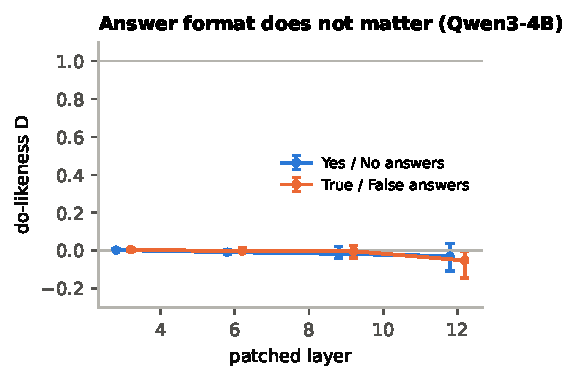
\includegraphics[width=0.85\columnwidth]{fig_tf.pdf}
\caption{Qwen3-4B, same 30 scenarios: median \D\ (95\% CI) with Yes/No and True/False answers.}
\label{fig:tf}
\end{figure}

\subsection{The cause is not copied in with the patch}
One trivial explanation for seeing-like patches is that the ``icy'' state already encodes ``snow''. Against this: the source stories never mention the cause, and removing it from the patch changes nothing. For each scenario we estimated a cause direction $\hat c$ (mean state with the cause stated true minus false) and removed its component from the patch's change, $\Delta' = \Delta - (\Delta\cdot\hat c)\hat c$. Over the 30 valid scenarios and layers 0--15 this shifts \D\ by at most 0.01 (all CIs within $-0.03$ to $+0.01$), the same as removing an unrelated scenario's direction; belief in the cause barely moves (2.26 $\to$ 2.21 at layer 12). The backward inference is computed downstream, as when the fact is read. Projection removes only linear overlap at one layer, so this rules out the simplest mechanism, not every one.

\subsection{Can a patch carry an intervention?}\label{sec:ds}
We copied the fact's state from the \textbf{do} story instead (``\dots the water froze, so the road was icy''), where the model has already read that an outside cause produced the fact. By the middle layers that state has absorbed its context (cosine similarity to the plain ``icy'' state falls from 0.998 at layer 0 to 0.905 at layer 13), yet patched into a neutral story it acts exactly like the plain version through most of the network (Table~\ref{tab:ds}, Fig.~\ref{fig:ds}). Only in the last 3--4 layers where patches still work does it move the model part of the way towards doing, in all four runs, and never near $D=1$.

\begin{table}[t]
\caption{Do-source patches: paired difference $D_\text{do}-D_\text{see}$.}
\label{tab:ds}
\centering\small
\setlength{\tabcolsep}{3pt}
\begin{tabular}{@{}lccc@{}}
\toprule
Run & $\approx0$ at & CI $>0$ at & Shift \\
\midrule
Qwen chains (30) & L0--13 & L14,16,17 & $+0.13$ to $+0.24$ \\
Qwen forks (9) & L0--9 & L12 & $+0.21$ \\
Llama chains (23) & L0--6 & L7,8,9 & $+0.35$ to $+0.48$ \\
Llama forks (9) & L0--6 & L9 & $+0.29$ \\
\bottomrule
\end{tabular}
\end{table}

\begin{figure}[t]
\centering
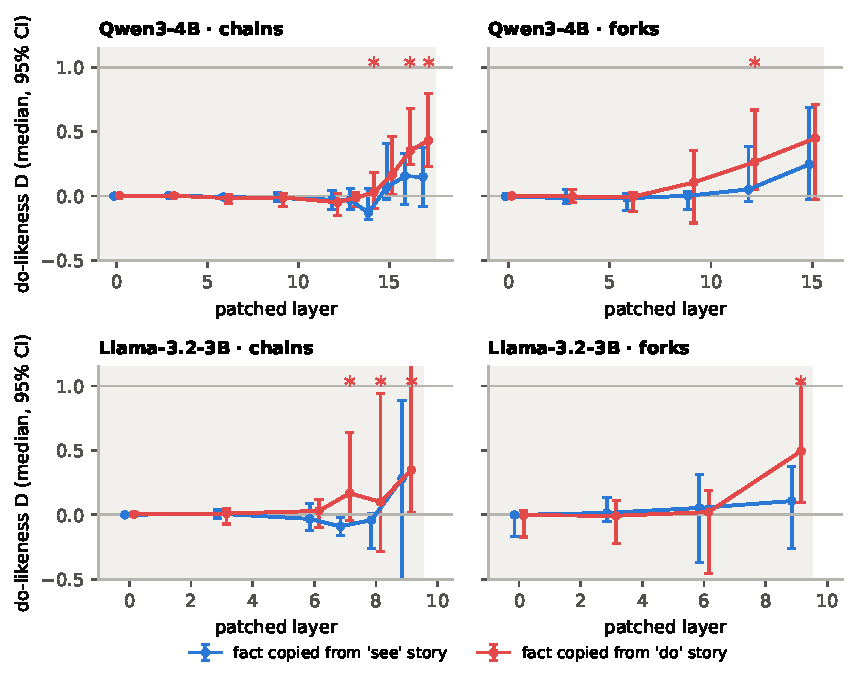
\includegraphics[width=\columnwidth]{fig_dosource.pdf}
\caption{Median \D\ (95\% CI) of word patches copied from the see story (blue) or the do story (red). Shaded: layers where the true patch passes. $\ast$: paired difference $\ge0.05$ with CI above 0.}
\label{fig:ds}
\end{figure}

\textbf{Pre-registered test (DS2).}\label{sec:ds2} The late shift was first seen in an exploratory run, so we repeated the experiment on 16 fresh variants of every valid scenario that had never been used for patching (Qwen: 480 items, 30 scenarios; Llama: 368 items, 23 scenarios), adding two patches. A \textbf{column patch} replaces the fact word at every layer $0..L$. A \textbf{reverse patch} writes the see-version of the word into the \emph{do} story: if knowledge of the intervention lives at the cause words, the do story should stay do-like. The text filters still held for 30/30 Qwen and 22/23 Llama scenarios, and the true patch passed at every tested layer. Four of five predictions held in full and the fifth in direction (Table~\ref{tab:ds2}, Fig.~\ref{fig:ds2}).

\begin{table}[t]
\caption{Pre-registered predictions for DS2 and outcomes.}
\label{tab:ds2}
\centering\footnotesize
\setlength{\tabcolsep}{2pt}
\begin{tabular}{@{}p{2.35cm}p{2.45cm}p{2.3cm}c@{}}
\toprule
Prediction & Qwen3-4B & Llama-3.2-3B & Held \\
\midrule
P1 early/mid: do-src = see-src & L0--12: $-0.01$ to $+0.02$ & L0--5: $-0.01$ to $+0.05$ & yes \\
P2 late: diff $\ge0.1$, CI$>0$ & L14--17: $+0.12,+0.13,$ $+0.19,+0.30$; 4/4 & L7--9: $+0.34,+0.47,$ $+0.54$; 3/3 & yes \\
P3 column $\ge$ single & same sign, $+0.12$ to $+0.26$, smaller & same sign, $+0.19$ to $+0.29$, smaller & part \\
P4 reverse stays do-like ($D\ge0.7$) & $D$ 0.94--1.00 (L0--13) & $D$ 0.93--1.00 (L0--5) & yes \\
P5 reverse drops late ($\ge0.1$) & to 0.77 col / 0.85 single & to 0.73 col / 0.86 single & yes \\
\bottomrule
\end{tabular}
\end{table}

\begin{figure*}[t]
\centering
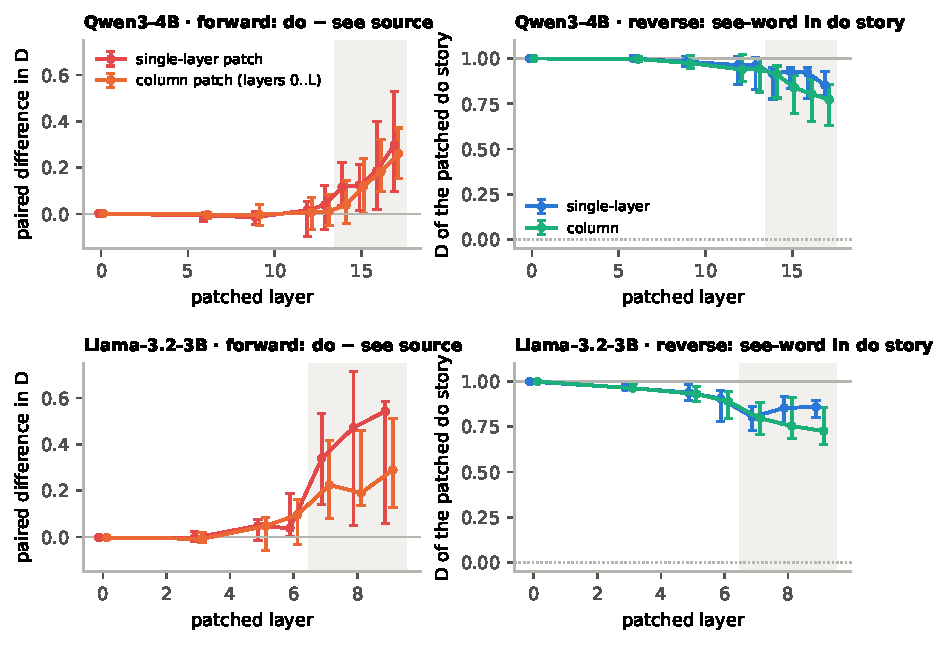
\includegraphics[width=0.78\textwidth]{fig_ds2.pdf}
\caption{Pre-registered test on fresh variants. Left: paired difference in \D\ between patching the fact word from the do story and from the see story (single-layer and column). Right: \D\ of the do story after its fact word is replaced by the see story's (1 = still fully do-like). Shaded: late layers named in the predictions.}
\label{fig:ds2}
\end{figure*}

Together: the knowledge that a fact was imposed is held at the cause words; from the last few working layers on, part of it is also carried at the fact's own position, but most of it never is.

%=====================================================================
\section{Discussion}
\textbf{Two levels of intervention.} A patch is a do() on the network and, in our experiments, an observation in the model's world. The two descriptions do not conflict, but they license different conclusions. Patching remains a sound tool for asking where information is held and which components matter. What it does not deliver is the effect of a fact in the model's world model: the downstream changes include everything the model infers from the fact, backward as well as forward.

\textbf{Why this is the natural outcome, and where it stops.} Downstream layers have only ever received a fact's state from text, so they treat it as they treat text. The do-source experiments mark the limit of this account: knowledge that a fact was imposed exists in the network, since the model reasons correctly about the imposed story, but for most of the depth it sits at the cause words. A fact's representation carries \emph{what} is true before it carries \emph{why}.

\textbf{Consequences for practice.} (i) A change in $Y$ after patching $X$ may reflect what $X$ is evidence for; probes of $X$'s causes separate the two. (ii) To make a model treat a fact as imposed, editing the fact's state is not enough; the cause positions must be edited too. (iii) In causal abstraction, an interchange intervention on a low-level state may implement \emph{conditioning} on the aligned high-level variable rather than do(); our score is one way to check which. (iv) Every yes/no read-out of an edited model needs unrelated-question controls.

\textbf{Addressing the review concern.} Edits can break language processing. Our pass rule guards against this: a patch is scored only if it moves the fact about as much as reading it does, beats an unrelated-story patch in $\ge70\%$ of scenarios (observed: 100\%), lowers belief when the source is false, and leaves unrelated questions unmoved ($\le0.21$).

%=====================================================================
\section{Limitations}
\textbf{Scenario selection:} edits are scored only where the model separates seeing from doing in text (30/45 chains for Qwen, 23 for Llama, 12 for Gemma), so claims cover scenarios the model handles correctly in text. \textbf{What ``doing'' means:} our do stories state an explicit outside cause, which the model may treat as an alternative explanation more than as an intervention in Pearl's sense; the do sentence is also longer than the see sentence. \textbf{Half the network:} single-position patches stop working at 35--50\% of depth; the late shift sits at the edge of this range, where single-layer estimates rest on few scenarios (5--24 in Qwen), although the column patch (26--28) agrees. \textbf{Scale and text:} three base models of 2--4B parameters, short template stories, single-token key words. \textbf{Coverage:} colliders on Qwen only; forks on Qwen and Llama; the pre-registered do-source test on chains, with fresh variants of the same scenarios. \textbf{Mechanism:} the projection test removes one linear direction at one layer.

\section{Conclusion}
Across three causal structures, three model families and two answer formats, a patched fact is treated as something the model has \emph{seen}: it infers the fact's usual cause and explains away rival causes, exactly as when it reads the fact. Knowledge that a fact was \emph{imposed} lives at the cause words and reaches the fact's position only late and partly. Patching is a do() on the network, but not on the world the network represents. Future work: patching cause words together with the fact, multi-position patches in later layers, and larger instruction-tuned models.

\section*{Reproducibility}
All code (17 GPU notebooks and a CPU notebook that rebuilds every figure from saved results), the dataset with its generator, all result files and the six pre-registration files are in the project folder submitted with this report.

\section*{Acknowledgment}
We thank Prof.\ Bhaskarjyoti Das and the ADA teaching assistants for feedback on the one-pager and review, and Kaggle and Google Colab for GPU time.

\begin{thebibliography}{99}\footnotesize
\bibitem{bigelow2025} E.~Bigelow, D.~Wurgaft, Y.~Wang, N.~Goodman, T.~Ullman, H.~Tanaka, and E.~S.~Lubana, ``Belief dynamics reveal the dual nature of in-context learning and activation steering,'' arXiv:2511.00617, 2025.
\bibitem{cohen2024} R.~Cohen, E.~Biran, O.~Yoran, A.~Globerson, and M.~Geva, ``Evaluating the ripple effects of knowledge editing in language models,'' \emph{Trans. ACL}, vol.~12, pp.~283--298, 2024.
\bibitem{dettki2025} H.~M.~Dettki, B.~M.~Lake, C.~M.~Wu, and B.~Rehder, ``Do large language models reason causally like us? Even better?'' arXiv:2502.10215, 2025.
\bibitem{dettki2026} H.~M.~Dettki, C.~M.~Wu, and B.~Rehder, ``Do LLMs share human-like biases? Causal reasoning under prior knowledge, irrelevant context, and varying compute budgets,'' arXiv:2602.02983, 2026.
\bibitem{feng2026} J.~Feng and F.~Rudzicz, ``CausalPrism: Component-level evaluation of intervention-based causal reasoning in large language models,'' in \emph{Findings of EMNLP}, 2026, pp.~27364--27389.
\bibitem{geiger2025} A.~Geiger \emph{et al.}, ``Causal abstraction: A theoretical foundation for mechanistic interpretability,'' \emph{J. Mach. Learn. Res.}, vol.~26, 2025.
\bibitem{heimersheim2024} S.~Heimersheim and N.~Nanda, ``How to use and interpret activation patching,'' arXiv:2404.15255, 2024.
\bibitem{joshi2026} S.~Joshi, A.~Mueller, D.~Klindt, W.~Brendel, P.~Reizinger, and D.~Sridhar, ``Causality is key for interpretability claims to generalise,'' arXiv:2602.16698, 2026.
\bibitem{makelov2024} A.~Makelov, G.~Lange, and N.~Nanda, ``Is this the subspace you are looking for? An interpretability illusion for subspace activation patching,'' in \emph{Proc. ICLR}, 2024.
\bibitem{meng2022} K.~Meng, D.~Bau, A.~Andonian, and Y.~Belinkov, ``Locating and editing factual associations in GPT,'' in \emph{Proc. NeurIPS}, 2022.
\bibitem{pearl2009} J.~Pearl, \emph{Causality: Models, Reasoning, and Inference}, 2nd~ed. Cambridge Univ. Press, 2009.
\bibitem{prakash2026} N.~Prakash, N.~Shapira, A.~S.~Sharma, C.~Riedl, Y.~Belinkov, T.~R.~Shaham, D.~Bau, and A.~Geiger, ``Language models use lookbacks to track beliefs,'' in \emph{Proc. ICLR}, 2026.
\bibitem{tanyel2026} T.~Tanyel and S.~Ayvaz, ``Whose effect is it? How objectives inflate learned subspace interventions,'' arXiv:2611.05033, 2026.
\bibitem{vig2020} J.~Vig, S.~Gehrmann, Y.~Belinkov, S.~Qian, D.~Nevo, Y.~Singer, and S.~Shieber, ``Investigating gender bias in language models using causal mediation analysis,'' in \emph{Proc. NeurIPS}, 2020.
\end{thebibliography}

\end{document}
